\documentclass{standalone}
\usepackage{tikz}
\begin{document}
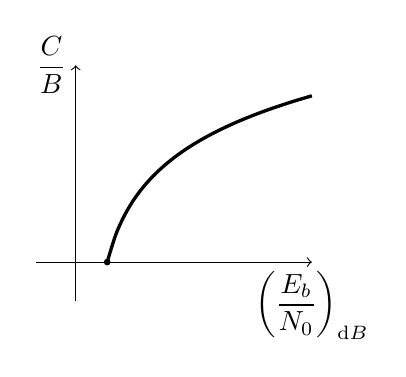
\begin{tikzpicture}[scale=2]
    \draw[->](-0.25,0)--(1.5,0)node[below]{$\displaystyle\left(\frac{E_b}{N_0}\right)_{\mathrm{d}B}$};
    \draw[->](0,-0.25)--(0,1.25)node[left]{$\displaystyle\frac{C}{B}$};
    \filldraw[black](0.2,0)circle(0.5pt);
    \draw[very thick, smooth, domain=0.2:1.5]plot(\x,{0.4*ln(10*(\x-0.1))});
\end{tikzpicture}
\end{document}